\chapter{Analisis de Resultados}

La construccion de la antena finalizo con todas las partes mecanicas y electronicas ensambladas. A continuacion se presentan los resultados obtenidos en la caracterizacion de la antena.\\

\begin{figure}
    \centering
    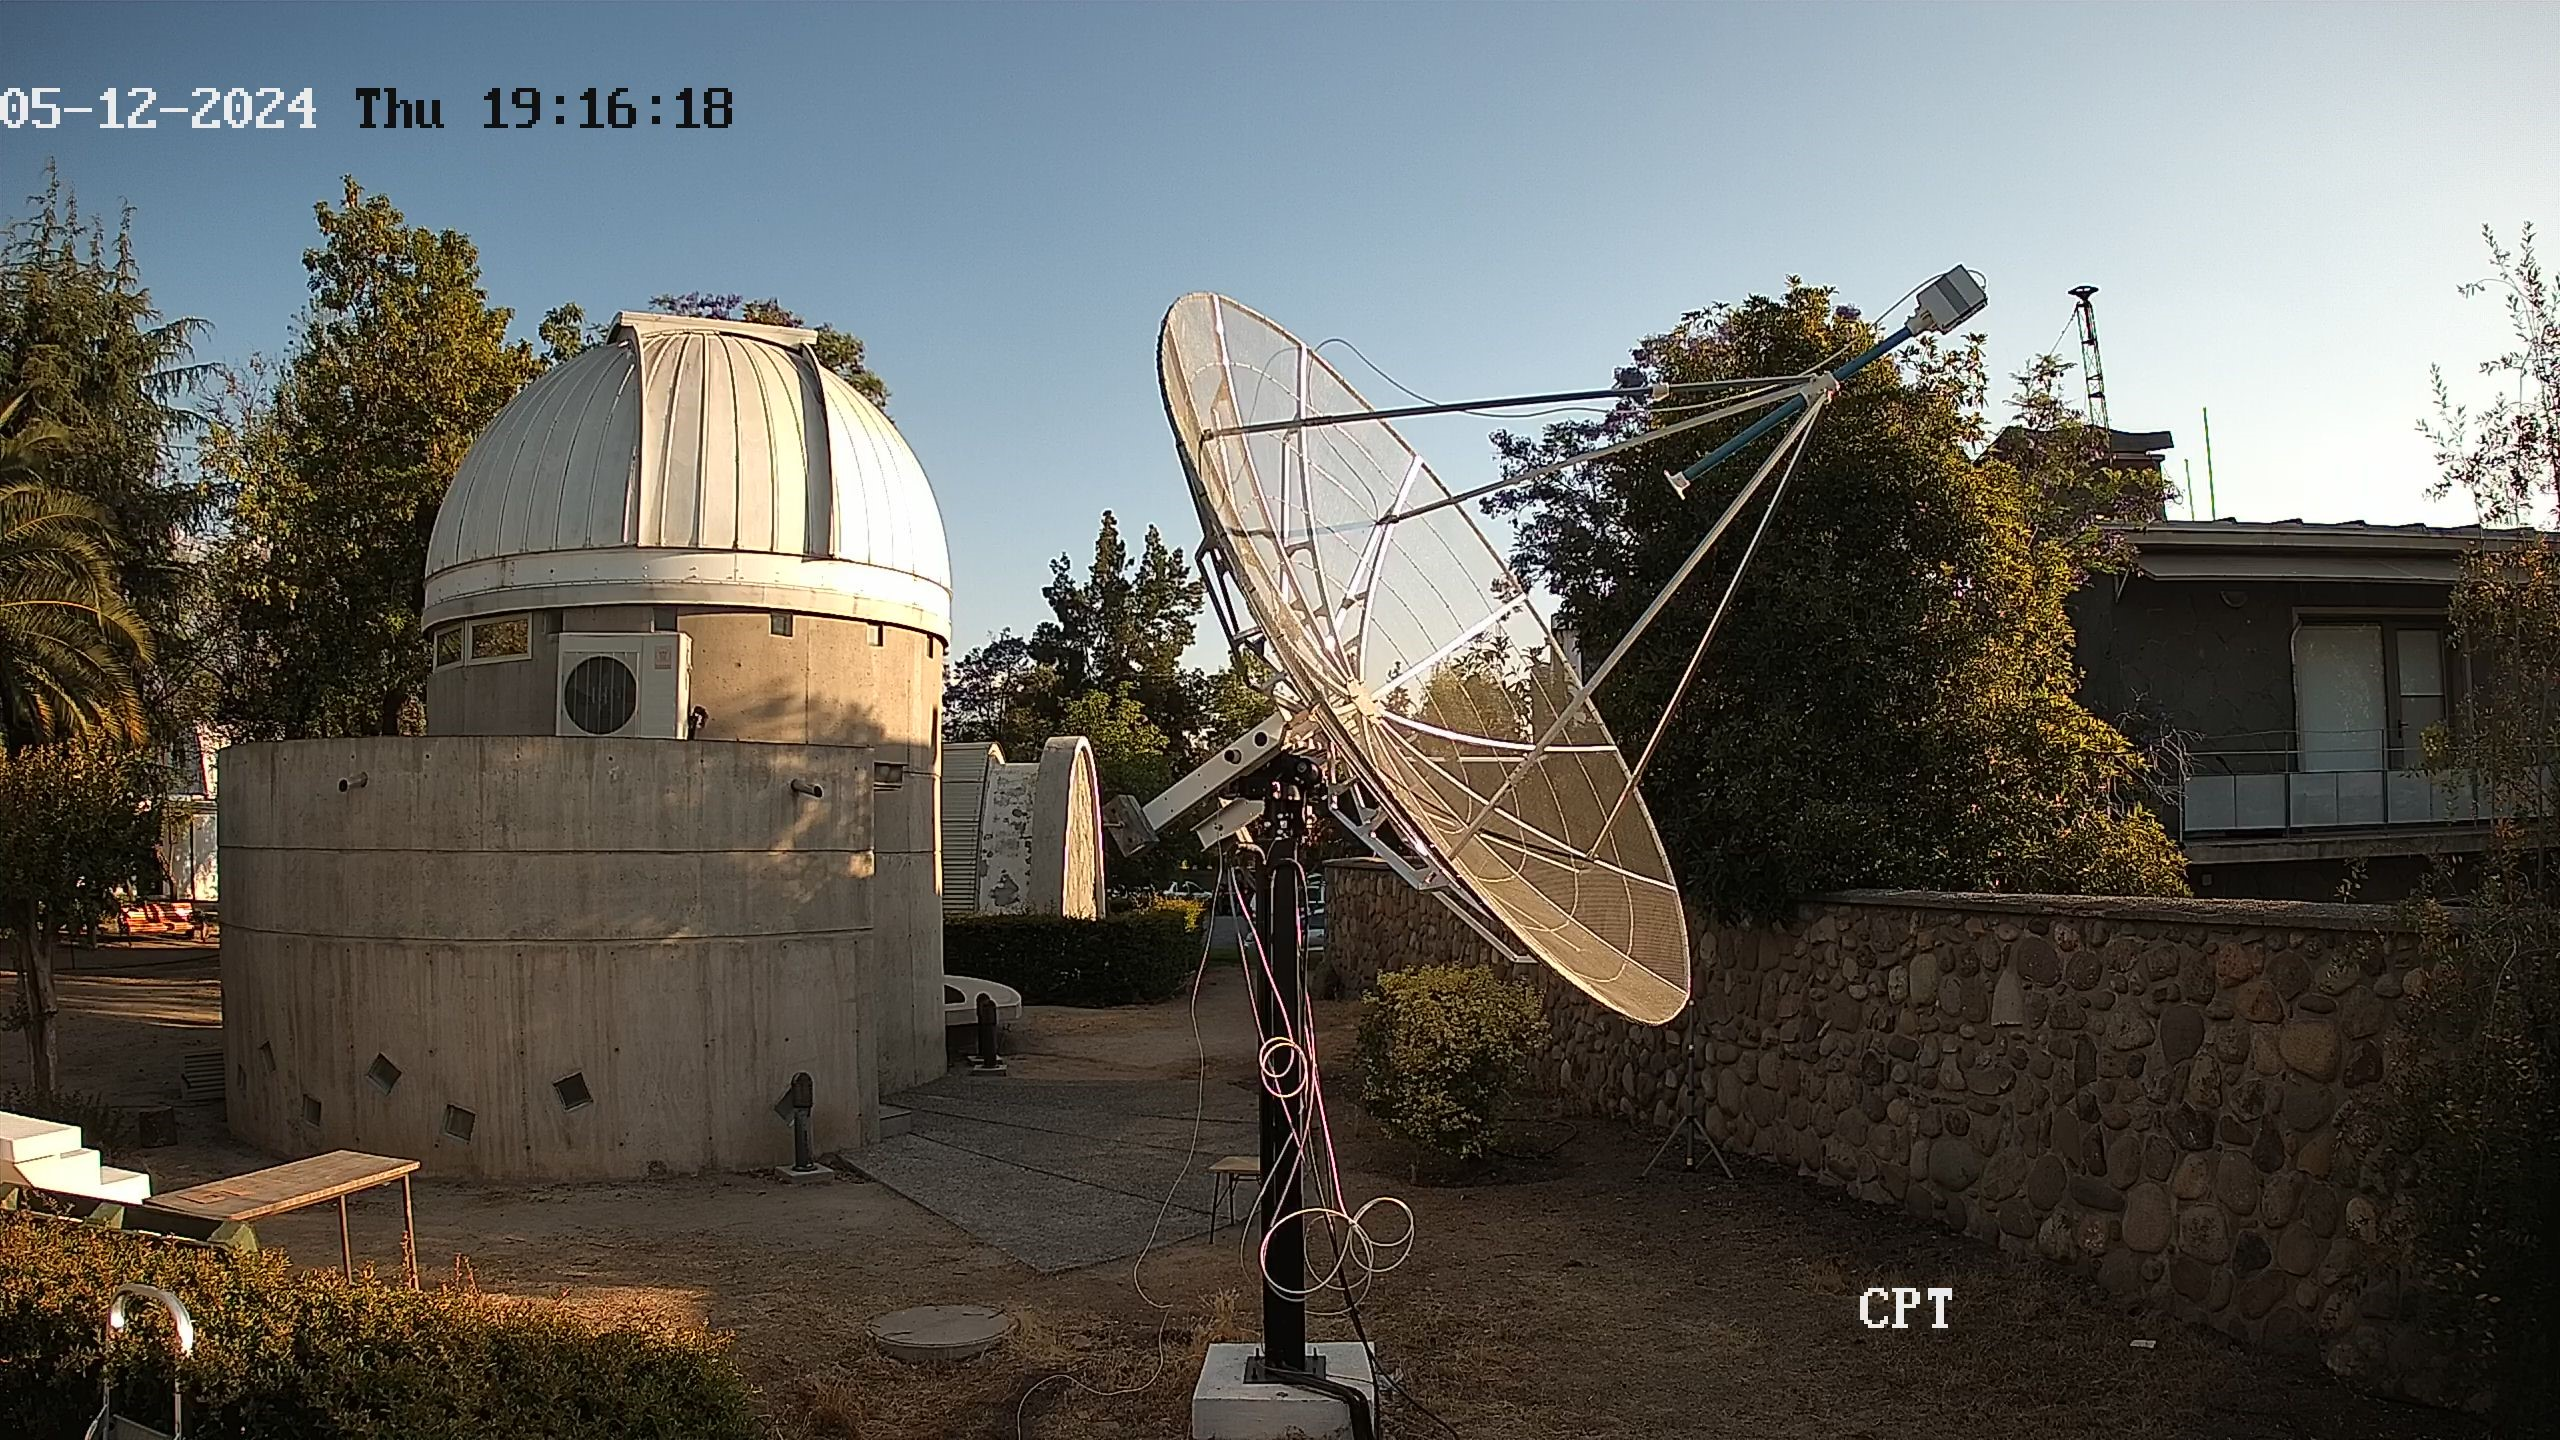
\includegraphics[width=0.8\textwidth]{img/antenna}
    \caption{Antena construida siendo monitoriada por la camara remota}
    \label{fig:antena}
\end{figure}

\section{Posicion del alimentador}

La posicion del alimentador con mayor ganancia se obtuvo a 135 cm de la superficie del reflector. La figura \ref{fig:distancia} muestra la ganancia en funcion de la distancia del alimentador al reflector.\\

La distancia obtenida coincide con la disatncia focal de la antena y se observa que la a medida que el alimentador se aleja del foco, aumentando o disminullendo la distancia con la parabola, la ganancia disminulle drasticamente perdiendo 6 dB por centimetro hasta llegar a la ganancia que tendria la antena sin considerar el reflector.\\

Estas perdidas se aprecian de la misma manera tanto para la frecuencia de 1428 MHz como para la de 400 MHz.\\

\section{Patrón de radiación}

A continuacion se presentan los patrones de radiacion obtenidos para la antena a 1428 MHz y 400 MHz. Para la banda de 1428 MHz se realizaron los 2 cortes de elevacion y azimut ya que este se obtuvo utilizando el digitalizador del receptor, lo que permite hacer las maniobras de elevacion completas. En cambio para 400 MHz, se debia utilizar un cable coaxial hacia el analizador de espectro.\\

% \begin{figure}
%     \centering
%     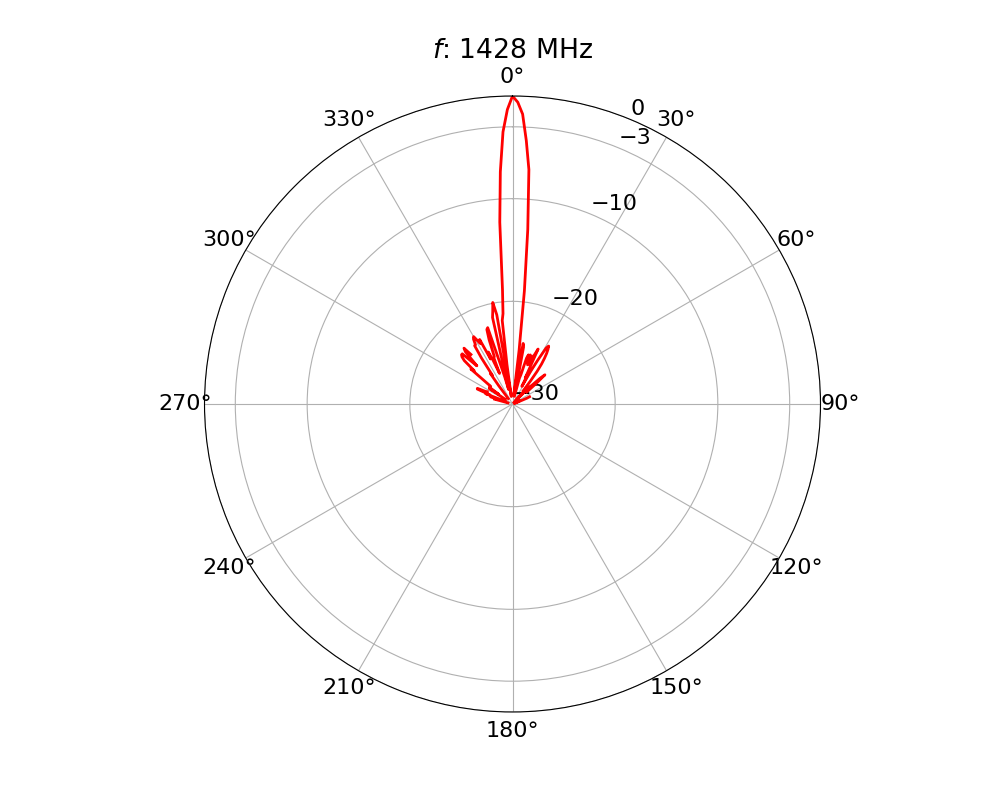
\includegraphics[width=0.8\textwidth]{img/1420rp}
%     \caption{Corte azimutal patrón de radiación a 1428 MHz}
%     \label{fig:1420rp}
% \end{figure}

% \begin{figure}
%     \centering
%     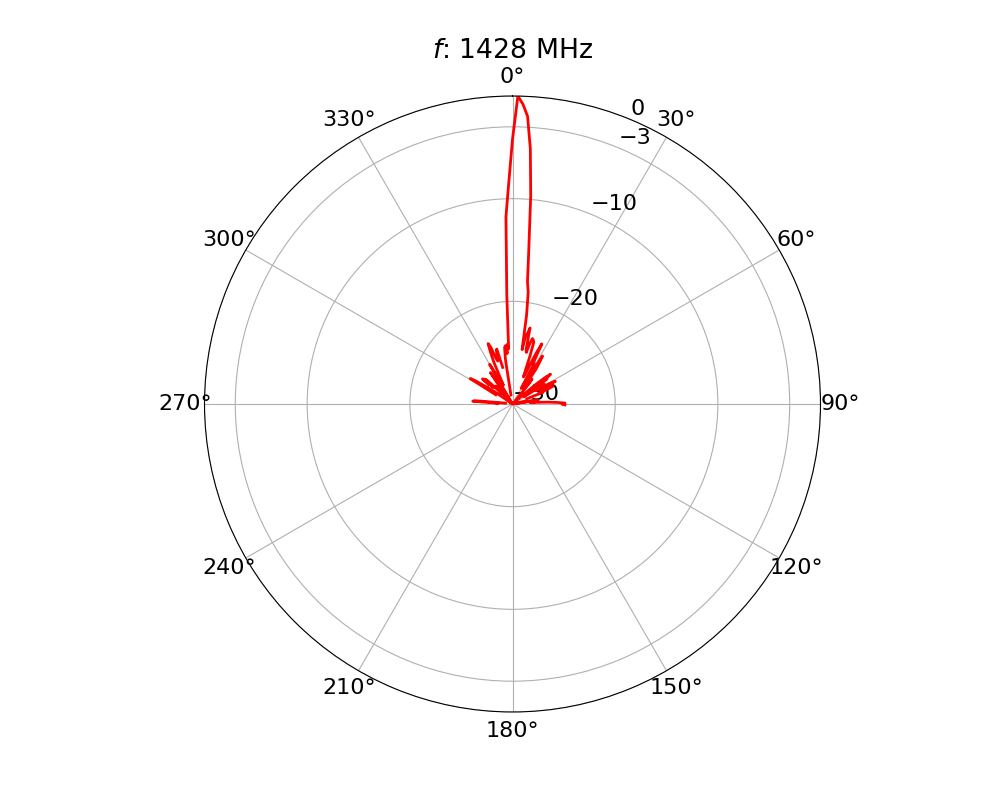
\includegraphics[width=0.8\textwidth]{img/1420rpel}
%     \caption{Corte elevacion patrón de radiación a 1428 MHz}
%     \label{fig:1420rpel}
% \end{figure}



\begin{figure}
    \centering
    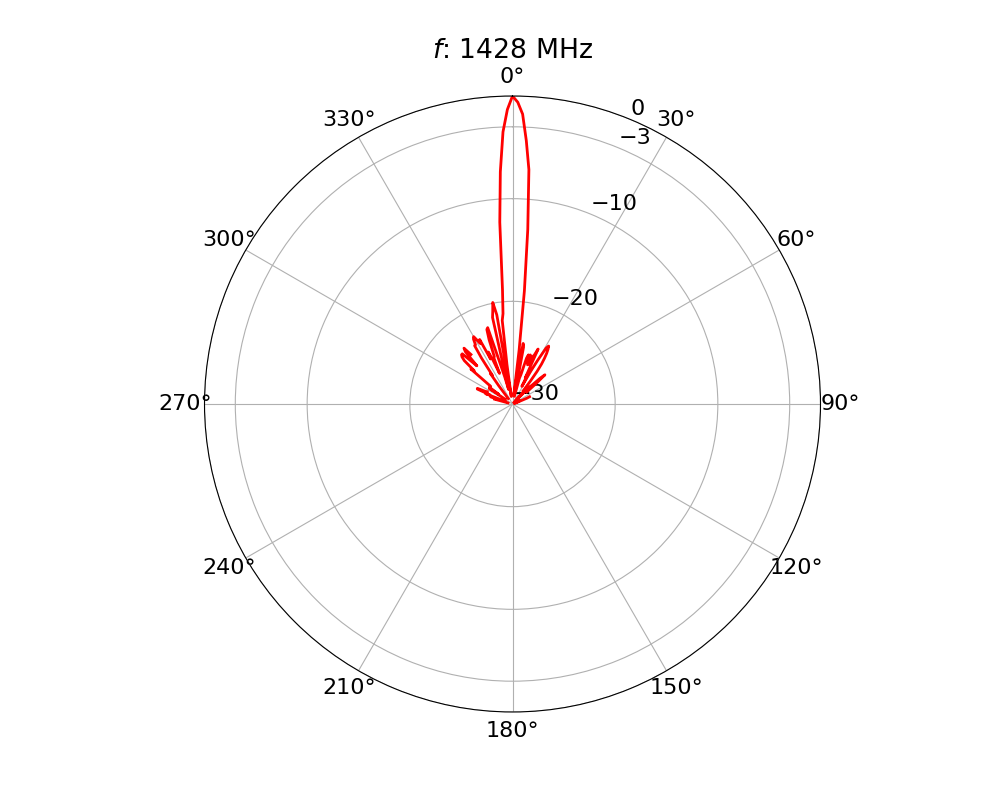
\includegraphics[width=0.8\textwidth]{img/1420rp}
    \caption{Corte azimutal patrón de radiación a 1428 MHz}
    \label{fig:1420rp}
\end{figure}

En la figura \ref{fig:1420rp} se observa el corte azimutal del patrón de radiación a 1428 MHz, donde se aprecia un lobulo principal predominante de 4.5 grados de HPBW y todos los demas lobulos laterales bajo -20 dB.\\

\begin{figure}
    \centering
    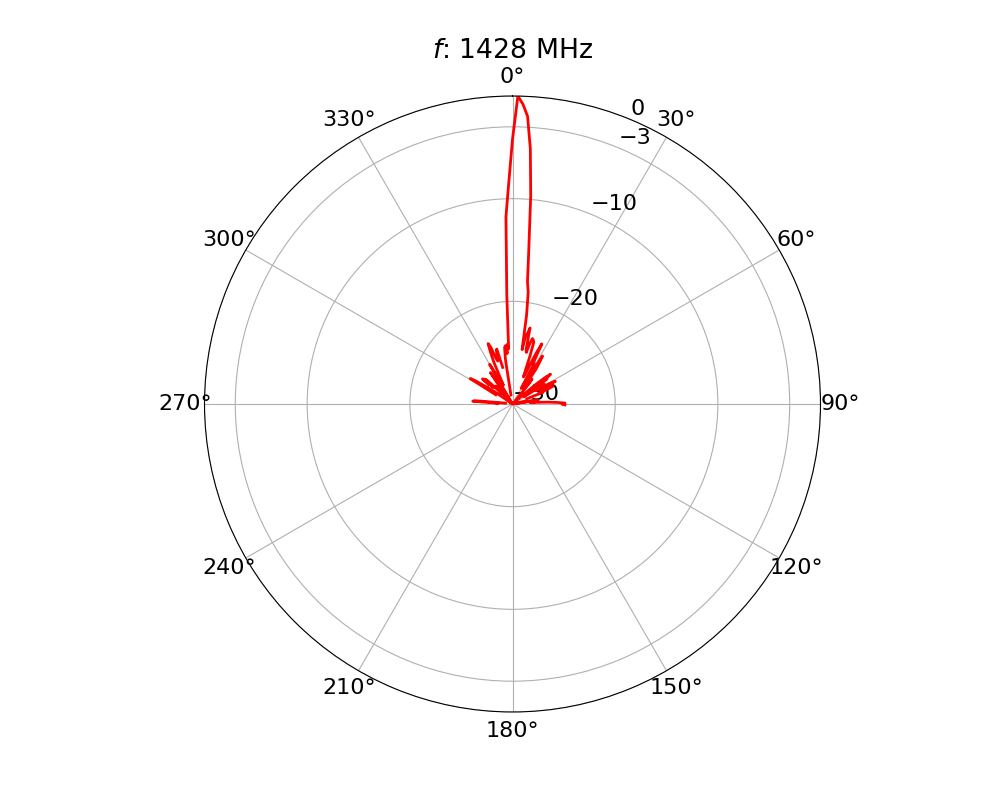
\includegraphics[width=0.8\textwidth]{img/1420rpel}
    \caption{Corte elevacion patrón de radiación a 1428 MHz}
    \label{fig:1420rpel}
\end{figure}

Con respecto al corte de elevacion, de la figura \ref{fig:1420rpel}, se observa un lobulo principal de 3.5 grados de HPBW y una discontinuidad en el lobulo principal a 0 grados. Los lobulos laterales  se encuentran por debajo de -25dB.\\

\begin{figure}
    \centering
    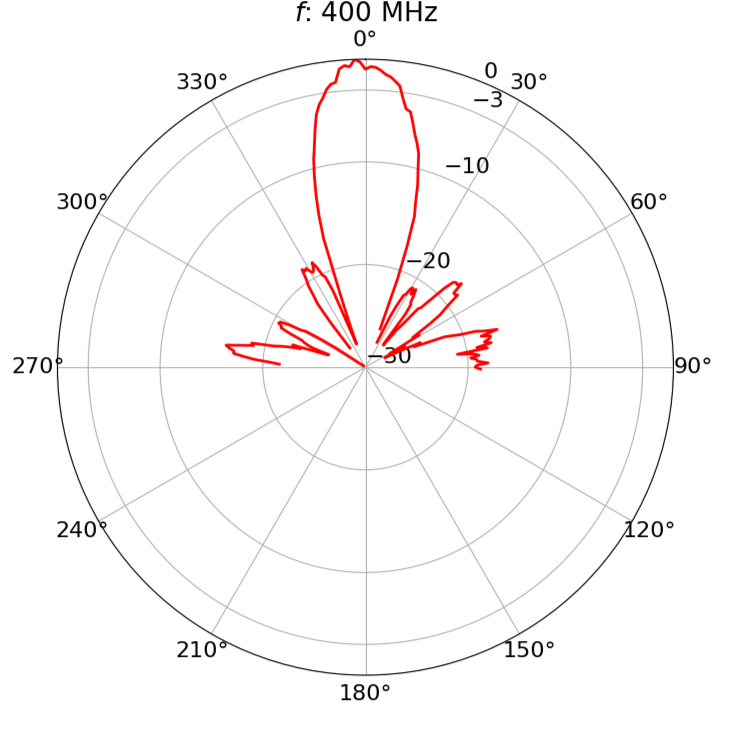
\includegraphics[width=0.8\textwidth]{img/400rp}
    \caption{Patrón de radiación a 400 MHz}
    \label{fig:400rp}
\end{figure}

\section{Ganancia y Directividad}



\section{Sensibilidad}

\section{Error de apuntamiento}

\section{Ancho de banda}

\section{Primera luz}